\section{Components Used}

\subsection{Microcontroller ATMega8}
Atmega8 is a high-performance, Low-power AVR, 8-bit Microcontroller with advanced \gls{risc} architecture. We have used ATmega8 to generate \gls{pwm} signals, to drive \gls{irled} and Ultrasonic sensors.
\begin{figure}[h!]
	\centering
	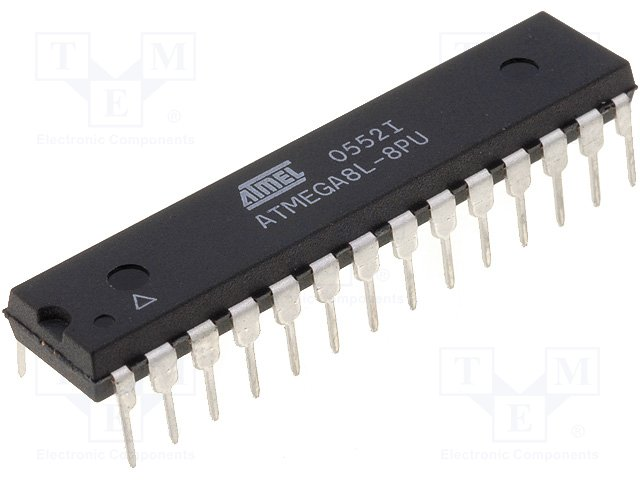
\includegraphics[scale=0.2]{Images/Atmega8.jpg}
	\caption{Microcontroller ATMega8}
	\label{fig:ATMega8}
\end{figure}

\subsection{Operational Amplifier}
UA741 operational amplifier is used in the system. UA741 is a general purpose operational amplifier and it can be used to amplify signal in the required range 40kHz. It is stable at this frequency range and has a stable response centered at this frequency.
\begin{figure}[h!]
	\centering
	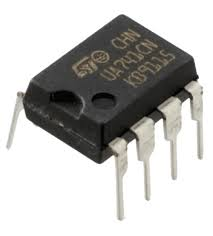
\includegraphics[scale=0.3]{Images/Opamp741.jpg}
	\caption{UA741 Operational Amplifier}
	\label{fig:Opamp741}
\end{figure}

\subsection{Tone Decoder}
IL567 Tone Decoder \gls{ic} is used in the system. This tone decoder is a general purpose tone decoder which looks for a close match between the frequency of incoming signal and of its internal oscillator. The frequency of it's internal oscillator can be controlled by adjusting the values of external capacitor and resistor connected to the IC. To filter out unnecessary signals picked up at the ultrasonic receiver we have used this IL567 Tone Decoder.
\begin{figure}[h!]
	\centering
	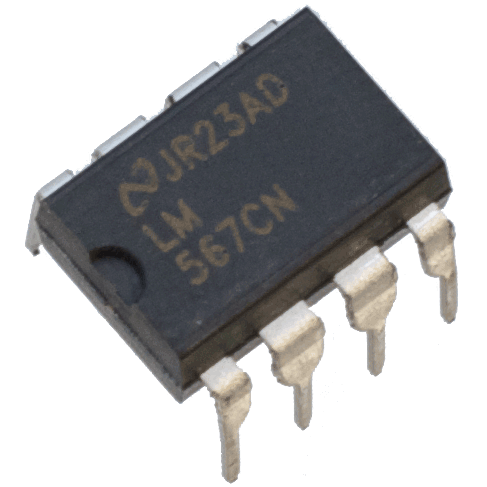
\includegraphics[scale=0.2]{Images/IL567.png}
	\caption{Tone Decoder IL567}
	\label{fig:IL567}
\end{figure}

\subsection{TSOP and \gls{irled}}
For the synchronization purpose we have used a pair of \gls{irled} and TSOP. \gls{irled} is used to send handshake signal which the TSOP detects and uses to synchronize the ultrasonic signal.

\begin{figure}[h!]
	\centering
	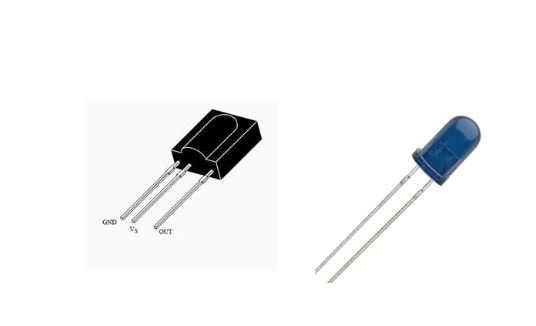
\includegraphics[scale=0.5]{Images/TSOPandIRLED.png}
	\caption{TSOP and \gls{irled}}
	\label{fig:TSOPandIRLED}
\end{figure}
